\chapter{Realizzazioni sperimentali e valutazione}
\label{capitolo4}
\thispagestyle{empty}

%Si mostra il progetto dal punto di vista sperimentale, le cose materialmente realizzate. In questa sezione si mostrano le attivit\`a sperimentali svolte, si illustra il funzionamento del sistema (a grandi linee) e si spiegano i risultati ottenuti con la loro valutazione critica. Bisogna introdurre dati sulla complessit\`a degli algoritmi e valutare l'efficienza del sistema.

%discorso sulla fisica e di tutti i valori?

\subsection{OSVR e le impostazioni iniziali}
\noindent Nei primi test eseguiti con l'OSVR appena installato, si è riscontrato un bug che, all'avviamento della simulazione, posizionava la telecamera ruotata di 90\degree verso destra e un inversione di rotazione tra roll (su Z) e pitch (su Y). La chiarificazione di questi movimenti si ha in figura \ref{fig:headmov}.
\begin{figure}[htb]
    \centering
    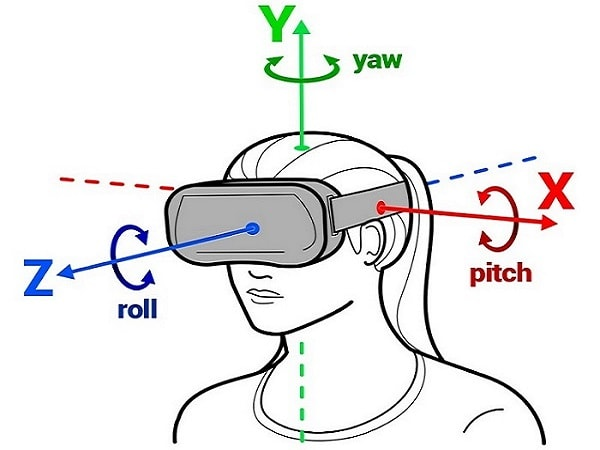
\includegraphics[height=8cm]{headmov}
    \caption{Le varie rotazioni della testa\label{fig:headmov}}
    \vspace{-0.3cm}
\end{figure}
\newpage
\noindent Il problema è che l'OSVR necessita di una calibrazione iniziale che non era stata eseguita dopo l'installazione. Si è risolto il problema posizionando la bicicletta a (0,0,0) con l'oggetto \textit{VRDisplayTracked} interno alla bicicletta con posizione (0,0,0) e tutte le rotazioni a 0. In questo modo le rotazioni a tempo di esecuzione erano tutte corrette.